% This is based on the LLNCS.DEM the demonstration file of
% the LaTeX macro package from Springer-Verlag
% for Lecture Notes in Computer Science,
% version 2.4 for LaTeX2e as of 16. April 2010
%
% See http://www.springer.com/computer/lncs/lncs+authors?SGWID=0-40209-0-0-0
% for the full guidelines.
%
%
%     To submit at ISWC 2018 - Resource Track
%
%
\documentclass{llncs}

\hyphenation{do-cu-ment do-cu-ments}

\usepackage[utf8]{inputenc}

\usepackage{graphicx}
\usepackage{comment}
\usepackage[usenames, dvipsnames]{xcolor}
\definecolor{igual}{rgb}{0.21, 0.11, 0} 
\usepackage{hyperref}
\definecolor{dark-blue}{rgb}{0.0,0.0,0.1}
\definecolor{dark-green}{rgb}{0.0,0.1,0.0}
\definecolor{dark-red}{rgb}{0.1,0.0,0.0}
\hypersetup{
    colorlinks, linkcolor={dark-red},
    citecolor={dark-green}, urlcolor={dark-blue},
    pdftitle={Multilingual Comparison of Entity Linking Systems},    % title
    pdfauthor={Henry Rosales-Méndez, Barbara Poblete and Aidan Hogan},     % author
    pdfsubject={LD4IE 2017},   % subject of the document
    pdfkeywords={multilingual;} {entity linking;} {information extraction;}, % list of keywords
}
\usepackage{amsmath}
\newcommand{\argmin}{\arg\!\min}
\newcommand{\argmax}{\arg\!\max}

%para el simbolo de chequeado
\usepackage{amssymb}% http://ctan.org/pkg/amssymb
\usepackage{pifont}% http://ctan.org/pkg/pifont
\newcommand{\cmark}{\ding{51}}%
\newcommand{\xmark}{\ding{55}}%

\usepackage{moreverb}% usar verbatim + box
\usepackage{breqn}

\usepackage{booktabs} 
\usepackage{multirow}

\usepackage{soul} %underline
\usepackage{pgfplots}
\begin{document}

\title{VoxEL: A Benchmark Dataset for Multilingual Entity Linking}
%
\titlerunning{}  % abbreviated title (for running head)
%                                     also used for the TOC unless
%                                     \toctitle is used
%
\author{Henry Rosales-M\'endez, Aidan Hogan and Barbara Poblete}
%
\authorrunning{Rosales-Méndez et al.} % abbreviated author list (for running head)
%
%%%% list of authors for the TOC (use if author list has to be modified)
%\tocauthor{Ivar Ekeland, Roger Temam, Jeffrey Dean, David Grove,
%Craig Chambers, Kim B. Bruce, and Elisa Bertino}
%
\institute{Center for Semantic Web Research, DCC, University of Chile \\
\texttt{\{hrosales,ahogan,bpoblete\}@dcc.uchile.cl}}

\maketitle              % typeset the title of the contribution
\begin{abstract}
%The Entity Linking (EL) task identify the entities mentions in a text corpus and associate them with corresponding entries in a knowledge base. Most EL approaches are suitable in the English context, but current trends are focused on agnostic-language approaches that allow us to perform EL over texts in many languages. One of the obstacles in multilingual contexts is that publicly available resources are scarce in multilingual contexts. This constitutes a hinder to achieve evaluation the quality of multilingual EL approaches, therefore, it is difficult to achieve progress in the area. In this work we propose VoxEL, a multilingual gold standard manually annotated that involve five languages that aim to favor the evaluation multilingual processes in EL. We also explore the behavior of state of the art of multilingual EL according to VoxEL and propose a new perspective to achieve multilingual annotations through automatic translation.

The Entity Linking (EL) task identifies entity mentions in a text corpus and associates them with corresponding entities in a knowledge base. While traditional EL approaches have largely focused on English texts, current trends are towards language-agnostic or otherwise multilingual approaches that can perform EL over texts in many languages. One of the obstacles to ongoing research on multilingual EL -- and in particular the evaluation of such systems -- is a scarcity of annotated datasets with the same text in different languages. In this work we thus propose VoxEL: a manually-annotated gold standard for multilingual EL featuring the same text expressed in five European languages. We first motivate and describe the VoxEL dataset. We then present the results of experiments using this dataset to compare the behavior of state of the art of (multilingual) EL systems across the five different languages, additionally comparing these results with methods using machine translation to English.
\keywords{Benchmark, Dataset, Multilingual Entity Linking}\\
\textbf{Resource type}: Dataset\\
\textbf{Permanent URL}:
\end{abstract}

\section{Introduction} 
\label{sec:intro}

%There is a large amount of textual information available in an unstructured format, that is understandable to humans but difficult to process automatically by machine. 
%The vast amount of unstructured textual information available makes it impossible to assimilate for human beings, so automatic techniques are necessary to process it. In this context, Entity Linking (EL) is a task of Information Extraction (IE) that aim to bring some notion of \textcolor{red}{structure} in textual corpora, identifying and linking entities in the text with their corresponding knowledge-base entries. 

The Entity Linking (EL) task identifies entity mentions in a text corpus and associates them with corresponding entities in a Knowledge Base (KB). In this way, we leverage the semantic information of publicly available KB about real-world entities to achieve a better understanding of natural language text. For instance, in the text \textit{``in the world of pop music, there is Michael Jackson and there is everybody else''} wrote in The New York Time, we can link the mention \textit{Michael Jackson} with its entry in Wikidata (\url{http://www.wikidata.org/entity/Q2831}), and thus, we can use all the knowledge behind this KB about Michael Jackson in our benefit. For this reason, EL is commonly used as support to other tasks that deal with natural language text and its underlaying semantic, among them semantic search, relationship extraction, text enrichment, entity summarization, semantic annotation, etc. 


%Currently there is a huge and variety of KBs available, the most popular have open domain , while others describe a specific areas of the knowledge such as Bioinformatics~\cite{UniProt2016kbbioinformatic}, Music~\cite{flabase2015musickbs}, Electromedicine~\cite{pdd2017electro_medical_kbs}, etc. This variate and 

One of the biggest motivations that have impulsed this task is the variety of KB that have been published in recent decades and that describe several real-live entities (e.g., Wikipedia, DBpedia, Wikidata). However, the decision to select an unambiguous entry in a KB to describe the correct meaning of a mention remains a challenge. One hand, due to the name variation issue that is commonly involved in textual information, i.e., that the same KB entry can be referred by different mentions. In the previous example, The New York Time should reference to Michae Jackson also as \textit{``Michael Joseph Jackson''} or \textit{``Jackson''}  and for all cases it should be linked to the same entity. On the other hand, a major obstacle is ambiguity, because a mention can refer to more than one candidate entry in a KB when only one is the appropriated. For instance, in Wikidata there are other person with the name \textit{``Michael Jackson''} such as a journalist (\url{https://www.wikidata.org/wiki/Q167877}), football player (\url{https://www.wikidata.org/wiki/Q6831558}), actor (https://www.wikidata.org/wiki/Q6831554) and others, which we have to deal with in the disambiguation process. 

%Another problem concerning to EL is the lack of consensus about the concept of ``entity''\cite{Borrega2007}. Some definitions of entity have been proposed in the literature by different areas of Natural Language Processes to response \textit{``what is an entity?''} but still remain an open issue~\cite{ourAMW2018}. As consequence, to decide when to select or not a mention for the annotation process is unclear in EL, as well as the inclusion or not of annotations in gold standards for evaluation purposes. In order to lessen this phenomenon Jha et al.~\cite{Jha2017} proposes a set of desirable properties that a gold standard must satisfy. On the other hand, \textcolor{red}{as we show in our previous work~\cite{ourAMW2018}}, we advocate for a more practical point of view inherent to EL that takes into account the domain of application rather a semantic perspective. Therefore, we encourage to answer better the question \textit{``what should Entity Linking link?''}. For Instance, coreferences are not so important if we want to find all documents about US singers, but relevant in extraction relation scenarios where many relations may be expressed in text with pronouns. \textcolor{red}{Two versions of this desirable behavior (relaxed and strict) would be fairer}. The popular EL system Babelfy\cite{Babelfy-moro2014entity} implements this criterion allowing us to specify if we only wish to annotate Proper Names, or include also concepts such as belt, bed, chair, table, etc.


Commonly, EL systems are monolingual approaches that only annotate texts written in one single language, in most of the cases English. Such approaches often use resources of a specific language such as Part-Of-Speech taggers and WordNet\footnote{\url{https://wordnet.princeton.edu}; April 1st, 2018}, that difficult the generalization of the same analysis to other languages. A more ambitious philosophy of EL searches approaches that deal with texts in a set of languages, a point of view that has gained the attention of the EL community. In this way, some popular contents include special track for multilingual entity linking such as TAC KBP\footnote{\url{https://tac.nist.gov/2013/KBP/}; April 1st, 2018}%, NTCIR\footnote{\url{http://ntcir.nii.ac.jp/CrossLink/}; April 1st, 2018} 
and SemEval 2015 Task 13\footnote{\url{http://alt.qcri.org/semeval2015/task13/}; April 1st, 2018}. Although these events represent an impulse to this task, the gold standards used in these evaluations are only available for the participant. More popular gold standards are provided (e.g., AIDA/CoNLL~\cite{aida2011}, DBpedia Spotlight Corpus\cite{mendes2011dbpedia}, KORE 50~\cite{kore50}) but commonly involve only English. Moreover, other multilingual datasets have differences cross language that could  introduce biases in the evaluation of linguistic-based approaches.

In this paper we propose the VoxEL datasets, a new gold standard manually annotated that involve German, English, Spanish, French and Italian languages. This datasets have the equivalent text in these five languages selected over a curated source of news, that leads to a more accurate evaluative process for those systems that base their models on lexical analysis. In addition we explore the behavior of some state of the art of multilingual EL systems according VoxEL.

\begin{comment}
In this paper we explore the state of the art of EL in a multilingual environment and proposing some new \textcolor{red}{ideas/resources to do better}. In particular, we propose VoxEL, a new gold standard manually annotated with equivalent text in five languages. VoxEL is built on curated text in all the languages, which leads to a more accurate evaluative process for those systems that base their models on grammatical analysis. In addition, we define VoxEL in two perspectives, a strict one that contains only those entities that undoubtedly must be annotated, and another relaxed one that also includes any Wikipedia entry\footnote{Except for the redirection and disambiguation pages.}. On the other hand, we study a new perspective to perform multilingual EL taking advantage of the automatic translation. 


We summarize our  contributions as follows:
\begin{itemize}
\item We propose that El can be evaluated from two perspectives: relaxed and strict.%, and in this way make allow comparisons adjusted to the application domain of the systems.
\item We propose VoxEL in a relaxed and strict perspective, a new gold standard involving the languages German, English, Spanish, French and Italian.
\item We explore the behavior of popular EL systems according VoxEL providing a rank for each of these languages.
\item We report evaluation of multilingual EL system in some of theirs supported languages 
\item We propose a new way to perform multilingual EL through automatic translations exploiting that VoxEL is based on curated text for each of these languages.
\item We study the behavior of some EL systems in languages that are not in their settings.
\end{itemize}
\end{comment}

The remainder of this paper is organized as follows. In Section \ref{sec:relatedWork} we begin with %some background on the EL process and multilingual resources that have emerged in the past few years (Section 2). We then present a survey of EL approaches that offer evaluation over multiple languages (Section 3). Next we present the results of our experiments comparing the performance of selected EL systems over equivalent texts in the English and Spanish languages (Section 4). We finish the paper by summarizing some main conclusions (Section 5).


%===============================================================
\section{Preliminaries}
\label{subsect:preliminaries}

Let $E$ be a set of entities in a KB and $M$ the set of mentions in a given natural text. The EL task establish a link between each $m\in{}M$ with its corresponding entity $e\in{}E$. In general, EL techniques are divided into two main phases: Entity Recognition (ER) and Entity Disambiguation (ED). In the first one the mentions of entities in the text are identified, problem directly relates to Named Entity Recognition (NER). The second phase associate each of these mentions with a unique identifier of the KB, process that is commonly broken down as follows:

\begin{description}
\item \textit{Candidate entity generation}:
For each mention $m\in{}M$ this stage selects the most probably subset of KB entities $E_m \subseteq E$ to be the correct meaning of it. Often, this process is based in keyword matching between the $m$ and the label of the entities in $E$.

\item \textit{Candidate entity ranking}: This stage is where the disambiguation is made. Once we have the candidate entities $E_m$ for each mention $m$, then $E_m$ is ranked according to the probability that each $ E_{m_i} $ describe the correct meaning of $m$.

\item \textit{Unlinkable mention prediction}:
Generally, it is expected that the knowledge bases are large enough to link all the entity mentions, however this does not happen in reality. In this stage are identified those mentions for which no entity in the KB corresponds to it, and then they are labeled \textit{NIL} (Not In Lexicon). 
\end{description}

Both phases of EL are conducted in different ways in the community. Most systems perform recognition first, and once the mentions are identified the disambiguation phase is applied to them. This systems are so-called End-to-End, and usually run popular NER tools to perform recognition~\cite{mendes2011dbpedia,Babelfy-moro2014entity}. Other approaches do both phases in a unified process, keeping close the decision of identifying and linking a mention~\cite{joinapproach2015}. On the other hand, a less employed approach is to assume that mentions have already been identified by some existing approach and wait for a text with the mentions specified~\cite{mag2017}.

%Structured KBs as Wikidata, gather in the same multilingual resource all the information about each entity for all the languages.
%\textcolor{blue}{ This is convenient for EL benchmark  due to the same entity will always have the same cross-languages link. Opposed to this, KBs such as Wikipedia and DBpedia managing different editions (or chapters) by entities in different languages (e.g.,......) that can introduce ...}
%
%===============================================================
\section{Related Work}
\label{sec:relatedWork}

%-----------------------------------------------------------
\subsection{Multilingual Systems}
%.................
%% 1) HABLAR COSAS DE MULTILINGUAL
Commonly, EL systems are monolingual approaches that only annotate texts written in one single language. In Table \ref{tab:multilingual_approaches} we show approaches that handle the annotation of mentions in text written on more than one language, available in some cases as demo in web pages, source code or REST API. As expected, a high-level inspection of the table shows that English is the most involved language, follow by Europeans languages such as German, Spanish, French, Dutch and Italian. We shall only consider in our experiments those systems that provide a working-RESP-API web service, constraining that the systems are performed in the environment designed and configured by the authors. In addition, we involve in the experiment sonly those systems that links entities from Wikipedia or related resources such  as  DBpedia or YAGO. With this characteristic we select the follow systems: DBpedia Spotlight, TagME, THD, AGDISTIS, BABELFY and FREME NER. 

\begin{table*}[th!]
\centering
\caption{Overview of multilingual EL approaches. The italicized approaches will be incorporated as part of our experiments.}
\label{tab:multilingual_approaches}
\setlength{\tabcolsep}{3pt}
\begin{tabular}{lccccr}
\toprule
\textbf{Name} &  \textbf{Year} & \textbf{Evaluated Languages} & \textbf{Demo} & \textbf{Src} & \textbf{API}\\ \midrule

KIM \cite{KIM-popov2004kim} & 2004 &English, French, Spanish&\cmark&\xmark&\cmark\\\midrule

SDA \cite{SDA-charton2011automatic}  & 2011 &English, French&\xmark&\xmark&\xmark\\\midrule

ualberta \cite{guo2012ualberta}& 2012 &English, Chinese&\xmark&\xmark&\xmark\\\midrule

HITS \cite{fahrni2012hits} & 2012 & English, Spanish, Chinese&\xmark&\xmark&\xmark\\\midrule

\textit{THD} \cite{THD-dojchinovski2012recognizing}  & 2012 &English, German, Dutch&\cmark&\cmark&\cmark\\\midrule 

\textit{DBpedia Spotlight} \cite{mendes2011dbpedia,daiber2013improving} & 2013  &English, Italian, Russian,&\cmark&\cmark&\cmark\\
& &Dutch, French, German,&&&\\
& &Spanish, Hungarian, Danish&&&\\\midrule

\textit{TagME} \cite{ferragina2010tagme} & 2013 & English, German, Dutch &\cmark&\xmark&\cmark\\\midrule

Wang-Tang \cite{wang2013boosting} & 2013 & English, Chinese&\xmark&\xmark&\xmark\\\midrule

\textit{AGDISTIS} \cite{usbeck2014agdistis,mag2017}& 2014 & English, German, Spanish&\cmark&\cmark&\cmark\\
& &French, Italian, Japanese,&&&\\
& &Dutch&&&\\\midrule

\textit{Babelfy} \cite{Babelfy-moro2014entity}& 2014 &English, Spanish, French &\cmark&\xmark&\cmark\\
& &German, Italian&&&\\\midrule

WikiME \cite{Cross-Lingual-Wikifier-tsai2016cross} & 2016 & English, Spanish, French,&\cmark&\xmark&\xmark\\
& &Italian, Chinese, German,&&&\\
& &Thai, Arabic, Turkish,&&&\\
& &Tamil, Tagalog, Urdu, Hebrew&&&\\\midrule

\textit{FREME NER}~\cite{freme-ner2016}&2016&English, German&\xmark&\cmark&\cmark\\\midrule
%& &French, Spanish, Russian&&&\\\midrule

FEL~\cite{FEL-pappu2017lightweight}& 2017 &English, Spanish, Chinese&\xmark&\cmark&\xmark\\\midrule

FOX~\cite{fox2017}&2017&English, German, Spanish,&\cmark&\cmark&\cmark\\
& & French, Dutch &&&\\

%&2016&IDIOMAS&\cmark&\cmark&\cmark\\
%& & French, Dutch &&&\\
\bottomrule
\end{tabular}
\end{table*}

DBpedia Spotlight is one of the most popular EL system, proposed firstly in~\cite{mendes2011dbpedia} to deal with English annotations. An extended version proposes in~\cite{daiber2013improving} to leverage the multilingual information of Wikipedia and DBpedia KBs to support several languages. They base their ER on some substring matching techniques, which are raked latter by a probabilistic model. Another multilingual system popular in the EL community is TagME~\cite{ferragina2010tagme} which uses anchor texts in the Wikipedia pages to identify the mentions in the text. The ranking stage is based mainly in the commonness and relatedness measures, the first describes how often an anchor text is associated with a Wikipedia page and the other the relation that each page of Wikipedia has with the remaining mentions. In TagME apply the same process over different versions of Wikipedia to achieve multilingual annotations. On the other hand, THD takes advantage of the Wikipedia Search API in the specific languages to perform the disambiguation of the mentions after having identified the mentions by ER tools.

Another popular approach is AGDISTIS\cite{usbeck2014agdistis} which only do the ED phase and that was proposed to be agnostic to the KB. A Recent study \cite{mag2017} extend this approach, adding some new features to improve its behavior in multilingual scenarios. The candidate of generation is mainly performed for indexes computed off-line from the target KB, and then the ranking stage selects the high-quality related entities in a graph built over KB entities and mentions. BABELFY~\cite{Babelfy-moro2014entity} is other graph-based approach, based on BabelNet~\footnote{\url{http://babelnet.org/}; April 1st, 2018}. BabelNet is a multilingual KB constructed over Wikipedia and WordNet, filling the gap of information between the different version of Wikipedia by automatic translation. The ER is performed for Babelfy identifying by a Part-of-Speech tagging technique, and selecting the candidate entities by string matching. Finally, they rank the entities by searching the densest subgraph that relates the KB entities and identified mentions. FREME NER delegates the identification to StanfordNER tool and applies the ranking according a the a most-frequent-sense criterion.


\subsection{Multilingual Datasets}
%.................
%3) HABLAR SOBRE LOS corpus actuales monolingues

The task of EL emerged recently as a consequence of the growth of large sources of information about entities such as Wikipedia. Therefore, the number of datasets that describe the ideal behavior of EL systems on text collection is insufficient, so-called gold standard. In Table \ref{tab:datasets} we survey the main of these datasets of the literature, describing in most of the cases English annotations. As we can observe in Table 1, only four of these are suitable in multilingual assessment, prevailing English. 

\begin{table}[tb!]
\centering

\caption{Survey of dataset for EL task. For multilingual datasets only we show the quantities corresponding to English data. We present the metadata about the relaxed and strict version of our dataset by VoxEL$_r$ and VoxEL$_s$ respectively. (Abbreviations: $|D|$ number of documents, $|S|$ number of Sentences, $|E|$ number of Entities, \textit{Mn} denotes that all entities was manually annotated.)}
\label{tab:datasets} 
\begin{tabular}{lccccc}
\toprule
\textbf{Dataset}~~~~~~~~~~~~~~~~~~ &~~~~$|D|$~~~~ &~~~~$|S|$~~~~&~~~~$|E|$~~~~&~~~\textbf{Mn}~~~&~\textbf{Languages}~\\\midrule
AIDA/CoNLL-Complete~\cite{aida2011} &1393    &22,137 &34,929  &\cmark  &EN \\\midrule
AIDA/CoNLL-Test A~\cite{aida2011}   &216     &3,466  &5,917   &\cmark  &EN \\\midrule
AIDA/CoNLL-Test B~\cite{aida2011}   &231     &3,684  &5,616   &\cmark  &EN \\\midrule
AIDA/CoNLL-Training~\cite{aida2011} &946     &14,987 &23,396  &\cmark  &EN \\\midrule
KORE50~\cite{kore50}                &50      &50     &144     &\cmark  &EN \\\midrule
IITB~\cite{IITB2009}                &103     &1,781  &18,308  &\cmark &EN \\\midrule
ACE2004~\cite{ace04}                &57      &-      &306     &\xmark &EN\\\midrule
%OKE challenge 2016                 &\xmark  &\cmark &\cmark  & &\xmark \\\midrule
AQUAINT~\cite{aquaint}              &50      &533    &727     &\xmark &EN \\\midrule
MSNBC~\cite{MSNBC07}                &20      &668    &747     &\xmark &EN \\\midrule
DBpedia Spotlight
\cite{mendes2011dbpedia}            &10      &58     &331     &\cmark &EN \\\midrule
N3-RSS 500~\cite{n3}                &1       &500    &1000    &\cmark  &EN \\\midrule
Reuters 128~\cite{n3}               &128     & -     &881     &\cmark  &EN \\\midrule
Wes2015~\cite{wes2015}              &331     & -     &28,586  &\cmark  & EN \\\midrule
%Derczynski                         &\xmark  &\xmark &\cmark  & &\cmark \\\midrule
News-100~\cite{n3}                  &100     &-      &1656    &\cmark  &DE \\\midrule
Thibaudet~\cite{renden2016}         &1       &3,807  &2,980   &\xmark  &FR \\\midrule
Bergson~\cite{renden2016}           &1       &4,280  &380     &\xmark  &FR \\\midrule
SemEval 2015 
Task 13~\cite{moro2015semeval}      &4       &137    &769     &\cmark &EN,ES,IT \\ \midrule
DBpedia Abstract
~\cite{abstracts2016}               &39,132  &-      &505,033 &\xmark &DE,EN,ES,FR, \\
                                    &        &       &        &       &IT,JA,NL \\\midrule
MEANTIME \cite{meantime2016}        &120     &597    &2,790   &\xmark &EN,ES,IT,NL \\\midrule 
VoxEL$_r$                           &15      &94     &674     &\cmark &DE,EN,ES,IT,FR\\\midrule  
VoxEL$_s$                           &15      &94     &204     &\cmark &DE,EN,ES,IT,FR\\ 
\bottomrule
\end{tabular}
\end{table}


Some of these datasets have been proposed in areas of IE and adapted to EL, among them AIDA/CoNLL\footnote{It is so-called AIDA-YAGO2.} that contains annotations of mentions previously recognized in the Conference on Computational Natural Language Learning (CoNLL) that took place in 2003. Similarly, ACE2004~\cite{ace04} is a subset of the ACE co-reference corpus~\cite{ace04_old} based on three languages but annotated only for English. 

EL Challenges have been a rich source of multilingual datasets such as TAC KBP and SemEval 2015 but commonly are only available for the participant network. %In particular, the multilingual datasets employed in the evaluation process on 
We could locate SemEval 2015 Task 13~\cite{moro2015semeval} but not any of the datasets of TAC KBP. SemEval 2015 Task 13 is built over a biomedical, math, computer and social domain and it is designed to support EL and WSD at the same time, containing annotations to Wikipedia, Babelfy and WordNet.
One major project to provide a large-scale training and evaluation corpora is DBpedia Abstract\footnote{\url{http://wiki-link.nlp2rdf.org/abstracts/}; April 1st, 2018}\cite{abstracts2016}, which include the annotation of the abstract section of Wikipedia pages in six languages. On the other hand, MEANTIME\footnote{\url{http://www.newsreader-project.eu/results/data/wikinews/}; April 1st, 2018} consist on 120 news articles from WikiNews \footnote{\url{https://en.wikinews.org/}; April 1st, 2018} with manual annotations of entities, events, temporal information and semantic roles. Additional, this dataset has information about the intra-document, cross-document event and entity coreferences of its document that make it a more complex dataset than the previous ones.

Involving more than one language is differently implemented by KBs. While Wikipedia separates the entities by languages, structured KBs such as Wikidata gather in the same multilingual resource all the information about each entity for all the languages supported. %BabelNet constitute other multilingual KB that follows this desirable property, constructed over Wikipedia but without the information conflict problems of it. The gap between the different editions of Wikipedia was filled in BabelNet mainly with automatic translation. 
Having information gathered in this way allow EL systems to use the same link to annotate the same mentions in different languages, but in an environment like Wikipedia there are two ways make the annotations. For a given text input written in a specific language $L$, either the approaches target the entities of the version of the language $L$ of the KB (e.g., DBpedia Spotlight, AGDISTIS), or target the English version of the KB whatever the language $L$ is.%\textcolor{red}{We refer to the second ways of annotation in this paper as \textit{cross-lingual} links (e.g., Tagme, Babelfy).}

Multilingual datasets constitute a major challenge when dispose of the same information in all the languages what requires a major annotation effort, but it also makes it possible to compare the behavior of a system in the different languages. MEANTIME and SemEval 2015 Task 13 follow this property, opposite to DBpedia Abstract that contains different information in each language due to the inequality that the Wikipedia versions have for its different languages. However, MEANTIME and SemEval 2015 Task 13 use the automatic translation from English to obtain the text in the other languages. Despite the tremendous progress made in automatic translation in the last years, it can happen that it introduces translation errors. In this context, approaches based on grammar or any linguistic information could be devalued. 

%TOur dataset VoxEL is built over curted achiving the annotation through five languages.



%===========================================================================
\section{VoxEL Dataset} \label{sec:survey}

We describe in this section the VoxEL Datasets, a gold standard for EL that target the Wikipedia entries and involve five languages: German, English, Spanish, French and Italian. VoxEL is based on the VoxEurop\footnote{\url{http://www.voxeurop.eu/}; April 1st, 2018}, a European newsletter that constitutes a curated source of text, what facilitates the identification of the same mentions by the different version of the datasets, as well as the same annotations. To the best of our knowledge, the current multilingual datasets are build based on automatic translation, which could introduce lexical errors. With VoxEL, we provide to the community a more refined way to evaluate the behavior of EL systems in the same independent-language context. 

Taking into consideration the lack of consensus about \textit{``what is an entity?''} we propose handle two points of view of the annotations for the same input text. First, a \textit{relaxed} version that includes any Wikipedia page that is not disambiguation or redirection. Second, a \textit{strict} version that points only to irrefutable Wikipedia entities, and that are person, organization or place. Thus we can measure the behavior of systems according to its application domain. Some systems have a general purpose and allow us to adapt to the application domain, for instance, DBpedia Spotlight allow us to specify the confidence and support parameters with use to decide which entity links. Although these two parameters allow adjustment to the context, they should be calibrated each time it changes. An idea closer to our objective is the behavior of Babelfy, which allows us to specify if we want to annotate only entities, or if we allow the inclusion of concepts.

While this newsletter is a valuable source of information curated in several European languages, there are sometimes small changes in the text that, although they adapt to each language, produce omissions or changes of entities that could affect the performance of multilingual EL systems, even more so for the relaxed version that contains easily-replaceable entities. In order to achieve the same number of sentences and annotations for each new (document), we applied small handcrafted transformations to homogeneous the text. The sentences that introduce new entities or deviate a bit from the information shown by the documents in the other languages are eliminated. The most common transformations were caused due to the use of proper names for some languages when pronouns were found in other versions of the documents. 

To create the annotation of mentions with URIs, we implemented a web tool\footnote{\url{https://users.dcc.uchile.cl/~hrosales/NIFify.html}} that allows us the entire process of the dataset construction in NLP Interchange Format (NIF)~\cite{nif2013}, as well as a friendly visualization of the annotations that bring some advantages in the revision phase. For each annotation we specify two links, one that targets the English Wikipedia entry, and other is related to the version of Wikipedia corresponding to the input-text language $L$. In case there was no an appropriate Wikipedia entry for an identified mention we use the URI \url{https://en.wikipedia.org/wiki/NotInLexico} variating according $L$.

VoxEL consists of 15 news (documents) from the multilingual newsletter VoxEurop, which has 94 sentences for each document of the relaxed version, that also contains 674 mentions annotated in each language. For the same documents and sentences, the strict version contains 204 mentions annotated. This desirable property of simultaneously has the same annotations in the different document for each language is not presented in MEANTIME and the SemEval dataset. For instance, the SemEval dataset has 758, 768 and 784 annotations in the English, Spanish and Italian version respectively, as well as MEANTIME that has 2790, 2729, 2709 and 2704 mentions in the English, Dutch, Italian and Spanish version. 

%============================================================================
\section{Experiments}

We conduct some experiment in order to explore the behavior of state of the art EL systems in both version of the VoxEL dataset. In particular, we are interested in the following questions:
\begin{itemize}
\item \textbf{RQ1}: How does EL performance differ between the languages German, English, Spanish, French and Italian using VoxEL? 
%\item \textbf{RQ_}: Do multilingual systems configured for a set of languages perform much better over VoxEL for these languages than monolingual systems not configured for them?
\item \textbf{RQ2}: Could automatic translation be used to achieve results similar to that achieved in the English language by monolingual systems applied to texts written in a language that does not have its configuration?
\item \textbf{RQ3}: Taking into account that the systems obtain a better performance for English, could the automatic translation overcome the results of such systems for the other languages that support VoxEL?.
\end{itemize}

To response RQ1 we ran the multilingual systems Babelfy, AGDISTIS, DBpedia Spotlight, FREME NER, TagME and THD over both version of VoxEL. The results are shown in Table~\ref{tab:gerbil}. We use these systems via their REST APIs maintaining its predetermined parameters, except for the case of Babelfy for which we analyze separately the inclusion (Babelfy$_r$) and not inclusion (Bablfy$_s$) of concepts in the annotations. This first experiment was conducted by designing a modified local version of GERBIL~\cite{gerbil2015}, which is a friendly platform with a suits of annotator and datasets available for agile comparisons. So far, GERBIL only consider English comparison, therefore, we include missing configurations in order that multilingual systems could annotate non-English texts. 


\begin{table}[tb!]
\centering
\caption{Evaluation of EL systems according GERBIL using Micro F$_1$. We refer FREME NER and DBpedia Spotlight as \textit{FREME} and \textit{DBspot} respectively. In the cases when no result was obtained we show $err$, as well as ``-'' when a system does not support the corresponding language.}
\label{tab:gerbil}
\begin{tabular}{@{}lcccccccccccc@{}}
%\begin{tabular}{@{}lllllllllll@{}}
\toprule
            && \multicolumn{5}{c}{Relax}   & \multicolumn{5}{c}{Strict}  \\ \midrule
            &&~~DE~~~&~~EN~~~&~~ES~~~&~~FR~~~&~~IT~~~&~~DE~~~&~~EN~~~&~~ES~~~&~~FR~~~&~~IT~~~\\
            \cmidrule(lr){3-7}\cmidrule(lr){8-12}
            &$mP$& 0,840& 0.649 & 0.835 & 0.824 & 0.810 & 0.932 & 0.785 & 0.929 & 0.889 & 0.907 \\
Babelfy$_r$ &$mR$& 0.181& 0.522 & 0.549 & 0.488 & 0.451 & 0.676 & 0.735 & 0.710 & 0.632 & 0.578 \\
            &$mF$& 0.595& 0.578 & 0.662 & 0.613 & 0.579 & 0.784 & 0.759 & 0.805 & 0.739 & 0.706 \\\midrule
            &$mP$& 0.903& 0.722 & 0.916 & 0.912 & 0.884 & 0.942 & 0.816 & 0.923 & 0.912 & 0.894 \\
Babelfy$_s$ &$mR$& 0.461& 0.219 & 0.210 & 0.200 & 0,192 & 0.558 & 0.524 & 0.593 & 0.563 & 0.583 \\
            &$mF$& 0.301& 0.336 & 0.342 & 0.328 & 0.316 & 0.701 & 0.638 & 0.722 & 0.697 & 0.706 \\\midrule
            &$mP$& 0.313& 0.348 & 0.437 & 0,282 & 0.512 & 0.568 & 0.779 & 0.549 & 0.475 & 0.725 \\
AGDISTIS    &$mR$& 0.237& 0.265 & 0.329 & 0,210 & 0,397 & 0.568 & 0.779 & 0.549 & 0.475 & 0.725 \\
            &$mF$& 0.270& 0.301 & 0.376 & 0.241 & 0.447 & 0.568 & 0.779 & 0.549 & 0.475 & 0.725 \\\midrule
            &$mP$& 0.731& 0.745 & 0.691 & 0.658 & 0.682 & 0.781 & 0,854 & 0.690 & 0.691 & 0.800  \\
DBspot      &$mR$& 0.508& 0.577 & 0.399 & 0.360 & 0.488 & 0.544 & 0.602 & 0.382 & 0.406 & 0.549  \\
            &$mF$& 0.600& 0.650 & 0.506 & 0.466 & 0.569 & 0.641 & 0.706 & 0.492 & 0.512 & 0.651 \\\midrule
            &$mP$& $err$& 0.771 & $err$ & $err$ & $err$ & $err$ & 0.872 & $err$ & $err$ & $err$  \\
FREME       &$mR$& $err$& 0.379 & $err$ & $err$ & $err$ & $err$ & 0.402 & $err$ & $err$ & $err$  \\
            &$mF$& $err$& 0.508 & $err$ & $err$ & $err$ & $err$ & 0.550 & $err$ & $err$ & $err$ \\\midrule
            &$mP$& 0.635& 0.754 & -     & -     & 0.494 & 0.875 & 0.946 & -     & -     & 0.742  \\
TagME       &$mR$& 0.232& 0.488 & -     & -     & 0.182 & 0.652 & 0.784 & -     & -     & 0.509  \\
            &$mF$& 0.340& 0.592 & -     & -     & 0.266 & 0.747 & 0.857 & -     & -     & 0.604 \\\midrule
            &$mP$& 0.831& 0.806 & -     & -     & -     & 0.857 & 0.809 & -     & -     & -     \\
THD         &$mR$& 0.109& 0.253 & -     & -     & -     & 0.352 & 0.647 & -     & -     & -     \\
            &$mF$& 0.194& 0.386 & -     & -     & -     & 0.500 & 0.719 & -     & -     & -    \\\bottomrule 
            
\end{tabular}
\end{table}

We show in Table~\ref{tab:gerbil} the Micro F$_1$ obtained in the experiment\footnote{The GERBIL results are available at \url{https://users.dcc.uchile.cl/~hrosales/ISWC2018_experiment_GERBIL.html}}. While DBpedia Spotlight and FREME NER show a similar behavior in both environment, Babelfy, AGDISTIS, TagME and THD are sensitives to the inclusion of entities that do not are persons, organizations or places. In all of the cases, the involved systems agree with the fact that the strict version of VoxEL better fits the task needs. 

Incorporating more than one language into an EL approach brings with it an increase in its complexity. For instance, WikiME uses a model based on word embedding, which includes a final step for each foreign language embeddings of projection to the English one. On the other hand, Babelfy exploits the sets of synonyms of BabelNet\footnote{\url{http://babelnet.org/} KB; April 1st, 2018}, called \textit{Babel synsets}, that groups words in different languages to achieve multilingual EL. According to our review, no system has used machine translation to address the language barriers in EL. Some work with automatic translation is done in related areas, such as cross-lingual ontology matching~\cite{fu2010} where the impact of the translation quality is stressed.

In this direction, we design a second experiment in order to study the behavior of these same approaches configured only for English over the non-English version of VoxEL by automatic translation to English. For the automatic translation we use Google translator\footnote{\url{https://translate.google.com/}; April 1st, 2018}. VoxEL contains links to the language for each of its versions and also to English, what makes it possible to evaluate automatic translations directly. However, when we apply the translation we lost the details of the annotation information that it is required by GERBIL, such as the translated mention, initial and final position of the mention, etc. For this reason, we implement our own benchmark that leaves out the mentions information of the evaluation process, only considering the match between the URIs of the gold standard and the system results. 

In Table \ref{tab:translations} we show the results of the second experiment, showing the MicroF$_1$ score obtained for each system over the version of VoxEL written in its five languages. We configure the system with English and ran then over the version of VoxEL in the original language $L$ and also in the translated version, with the aim of having a point of reference that allows to mediate a worse and better behavior of the system on VoxEL. We took the first of both performances as \textit{base line} for each system and the second one as \textit{desirable performance}. As we can observe in Table~\ref{tab:translations}, the score from EL applied for the translation is between both criteria in all the cases, which indicates that the incorporation of automatic translation in this context obtains reasonable results. Thus, we respond the RQ2.


\begin{table}[tb!]
\centering
\caption{Performance of some EL systems using automatic translation according to $F_1$. For each system $Sys$ and the current language $L$ we show three experiments, first (\_,\_) denotes the behavior of $Sys$ configured with $L$ over the dataset wrote in this same language. The second (EN,EN$_t$) shows the results that involve the system $Sys$ configured with English and applied over an automatic translation of the datasets written in the current language to English. The third, denoted by (EN,\_), corresponds to the evaluation of $Sys$ configured with English and applied over the datasets written in the current language $L$. The information below to each system name correspond to (EN,EN) evaluation for the relax and strict version of VoxEL, in this order. }
\label{tab:translations}
%\begin{tabular}{@{}llllllllll@{}}
\begin{tabular}{@{}llcccccccc@{}}
\toprule
&             & \multicolumn{4}{c}{Relax}     & \multicolumn{4}{c}{Strict}    \\ \midrule
&             &~~~DE~~~&~~~ES~~~&~~~FR~~~&~~~IT~~~&~~~DE~~~&~~~ES~~~&~~~FR~~~&~~~IT~~~  \\ \cmidrule(lr){3-6}\cmidrule(lr){7-10} 
\multirow{3}{*}{\begin{tabular}[c]{@{}l@{}}Freme NER\\ (0.407,0.708)\end{tabular}}
& (\_,\_)     &0.282      &0.302      &0.268      &0.373      &0.483      &0.583      &0.479      &\ul{\bf 0.726}\\
& (EN,EN$_t$) &\ul{0.404} &\ul{0.403} &\ul{0.401} &\ul{0.408} &\ul{0.701} &\ul{0.713}&\ul{0.692} &0.711\\
& (EN,\_)     &0.166      &0.183      &0.196      &0.222      &0.190      &0.338      &0.342      &0.374\\ \midrule
\multirow{3}{*}{\begin{tabular}[c]{@{}l@{}}TagME\\ (0.462,0.327)\end{tabular}}
& (\_,\_)     &0.414      &-          &-          & -         &0.272      &-          &-          &-     \\
& (EN,EN$_t$) &\ul{0.431} &\ul{\bf 0.450}&\ul{0.441}&\ul{0.439}&\ul{0.330}&\ul{0.333} &\ul{0.321} &\ul{0.336} \\
& (EN,\_)     &0.188      &0.181      &0.200      &0.148      &0.212      &0.202      &0.197      &0.164 \\ \midrule
\multirow{3}{*}{\begin{tabular}[c]{@{}l@{}}DBspot\\ (0.466,0.707)\end{tabular}}
& (\_,\_)     &0.400      &0.331      &0.240      &0.342      &0.510      &0.477      &0.481      &0.653 \\
& (EN,EN$_t$) &\ul{0.441}&\ul{0.454}&\ul{0.464}&\ul{0.449} &\ul{0.696} &\ul{0.694} &\ul{0.721}&\ul{\bf 0.729} \\
& (EN,\_)     &0.209      &0.161      &0.18       &0.188      &0.374      &0.259      &0.326      &0.323 \\ \midrule
\multirow{3}{*}{\begin{tabular}[c]{@{}l@{}}THD\\ (0.392,0.625)\end{tabular}}
& (\_,\_)     &0.241      &-          &-          &-          &0.546      &-          &-          &-     \\
& (EN,EN$_t$) &\ul{0.394} &\ul{0.392} &\ul{0.386} &\ul{0.387} &\ul{0.597} &\ul{0.620} &\ul{0.595} &\ul{\bf 0.623} \\
& (EN,\_)     &0.207      &0.175      &0.217      &0.174      &0.251      &0.332      &0.403      &0.352 \\ \midrule
\multirow{3}{*}{\begin{tabular}[c]{@{}l@{}}Babelfy$_r$\\ (0.545,0.319)\end{tabular}}
& (\_,\_)     &\ul{0.523} &\ul{\bf 0.541}&0.493   &\ul{0.504} &\ul{0.344} &\ul{0.362} &0.309      &\ul{0.365} \\
& (EN,EN$_t$) &0.507      &0.515      &\ul{0.505} &0.501      &0.298      &0.298      &\ul{0.314} &0.301 \\
& (EN,\_)     &0.215      &0.170      &0.195      &0.140      &0.253      &0.239      &0.220      &0.179 \\ \midrule
\multirow{3}{*}{\begin{tabular}[c]{@{}l@{}}Babelfy$_s$\\ (0.308,0.567)\end{tabular}} 
& (\_,\_)     &0.279      &\ul{0.325} &0.290      &\ul{0.311} &\ul{0.572} &\ul{0.611} &\ul{0.583} &\ul{\bf 0.616} \\
& (EN,EN$_t$) &\ul{0.311} &0.309      &\ul{0.322} &0.303      &0.518      &0.523      &0.559      &0.532 \\
& (EN,\_)     &0.201      &0.179      &0.189      &0.137      &0.376      &0.372      &0.395      &0.258 \\ %\cmidrule(l){2-10} 
\bottomrule
\end{tabular}
\end{table}


%We underlined on in Table~\ref{tab:translations} for each system those scores that represent a better performance through automatic translation than with it own multilingual model. As we can observe, this happens for all the systems, at least for one of the languages.  In particular for DBpedia Spotlight this always happens. On the other hand, we also highlight with bold those scores that represent a better performance through automatic translation with respect the system configured for English over the English version, and we can see that the majority of these systems have this behavior according to VoxEL. So, this response RQ3, placing automatic translation as an option to tackle multilingual EL from systems with missing languages in their configuration as is the case of TagME and THD in this experiment. 

We underlined on in Table~\ref{tab:translations} for each system those scores that represent a better performance through automatic translation than the baseline and the desirable performance. As we can observe, this happens for all the systems, at least for one of the languages. In particular for DBpedia Spotlight, TagME and THD this always happens. On the other hand, we also highlight with bold font those scores that represent for each system the better performance among all its scores. This behavior is presented by three of the six systems considered in the experiment. So, this response RQ3, placing automatic translation as an option to tackle multilingual EL from systems with missing languages in their configuration as is the case of TagME and THD in this experiment. 

To give a better idea of the results obtained from the second experiment, we show in Figure~\ref{fig:bars} the average score of the selected systems in each of the languages supported by VoxEL. In both version of VoxEL we can observe that in average, the automatic translation is a way of approaching multilingual EL comparable with models that become more complex when they support more than one language. 

\begin{figure}
\caption{Average of the MicroF$_1$ evaluation that has the systems selected in each language supported by VoxEL, over its both version: (a) relaxed and the (b)strict. We show the \textit{Calibrated} values corresponding to the performance of each system configured by the current language, over the versions of VoxEL written in this same language. On the other hand, the \textit{Translation} and \textit{English} values are relating to the performance of each language configured for English and applied over the translation of version written in the current language to English and over the English version of VoxEL respectively.}
\label{fig:bars}
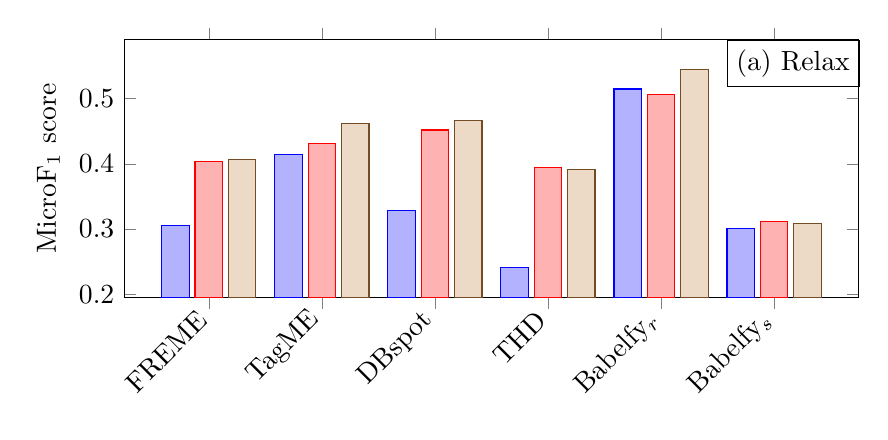
\begin{tikzpicture} 
\begin{axis}[ 
   title=(a) Relax,every axis title/.style={below right,at={(0.82,1)},draw=black,fill=white},
   ybar, 
   enlargelimits=0.15, 
   height=.4\textwidth,
   width=.9\textwidth,
   %legend style={at={(0.295,1)}, anchor=north,legend columns=-1}, 
   ylabel={MicroF$_1$ score}, 
   symbolic x coords={FREME,TagME,DBspot,THD, Babelfy$_r$,Babelfy$_s$}, 
   xtick=data, 
   %nodes near coords, 
   %nodes near coords align={vertical},
   x tick label style={rotate=45,anchor=east},
   %title=(relax)
 ] 
 \addplot coordinates {(FREME,0.306) (TagME,0.414) (DBspot,0.328) (THD,0.241) (Babelfy$_r$,0.515) (Babelfy$_s$,0.301)};
 \addplot coordinates {(FREME,0.404) (TagME,0.431) (DBspot,0.452) (THD,0.394) (Babelfy$_r$,0.507) (Babelfy$_s$,0.311)};
 \addplot coordinates {(FREME,0.407) (TagME,0.462) (DBspot,0.466) (THD,0.392) (Babelfy$_r$,0.545) (Babelfy$_s$,0.308)};
 %\legend{Calibrated,Translation,EN}
 \end{axis} 
\end{tikzpicture}


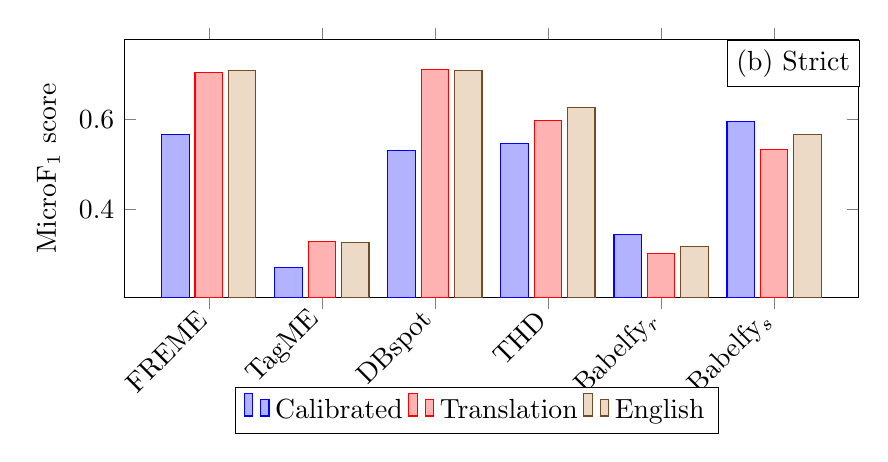
\begin{tikzpicture} 
\begin{axis}[ 
   title=(b) Strict,every axis title/.style={below right,at={(0.82,1)},draw=black,fill=white},
   ybar, 
   enlargelimits=0.15, 
   height=.4\textwidth,
   width=.9\textwidth,
   legend style={at={(0.48,-0.35)}, anchor=north,legend columns=-1}, 
   ylabel={MicroF$_1$ score}, 
   symbolic x coords={FREME,TagME,DBspot,THD, Babelfy$_r$,Babelfy$_s$}, 
   xtick=data, 
   %nodes near coords, 
   %nodes near coords align={vertical},
   x tick label style={rotate=45,anchor=east},
   %title=(relax)
 ] 
 \addplot coordinates {(FREME,0.567) (TagME,0.272) (DBspot,0.530) (THD,0.546) (Babelfy$_r$,0.345) (Babelfy$_s$,0.595)};
 \addplot coordinates {(FREME,0.704) (TagME,0.330) (DBspot,0.710) (THD,0.597) (Babelfy$_r$,0.302) (Babelfy$_s$,0.533)};
 \addplot coordinates {(FREME,0.708) (TagME,0.327) (DBspot,0.707) (THD,0.625) (Babelfy$_r$,0.319) (Babelfy$_s$,0.567)};
 \legend{Calibrated,Translation,English}
 \end{axis} 
\end{tikzpicture}
\end{figure}
%===============================================================
\section{Conclusion}
\label{sec:conclusion}

There are several multilingual approaches to address EL in the literature, as well as benchmark datasets that serve as a gold standard in the evaluation process. In this work we propose a manually annotated VoxEL, a new dataset that meets a set of properties that we consider desirable in multilingual EL assessments. Among these properties, we have that VoxEL has notes on cured texts, and not on texts translated automatically as is the case of some multilingual datasets of literature. This benefits to a greater extent to evaluate in a fair way the system that bases its models on intrinsic aspects of the lexicon. Also, we advocate for multilingual datasets that contain the same number of documents, sentences and annotations, in order to provide results that allow us the intra-language behavior of the systems. Property fulfilled by VoxEL.

We then conduct experiments to compare the performance of selected multilingual EL systems over VoxEL. We found an expected behavior in systems, being Babelfy and DBpedia Spotlight the best scored. In general, all the systems obtained better quality in the results for the annotations that only target persons, organizations and places. We also conducted experiments using VoxEL, to study how these systems perform when they are configured for the English language and an automatic translation is used to achieve multilingual annotation. 


{\footnotesize
\paragraph{Acknowledgements} The work of Henry Rosales-M\'endez was supported by CONICYT-PCHA/Doctorado Nacional/2016-21160017. The work was also supported by the Millennium Nucleus Center for Semantic Web Research under Grant NC120004. \textcolor{red}{We would like to thank Michael R\"oder for response some helpful email about GERBIL functionalities.}}

%
% ---- Bibliography ----
%
%\bibliographystyle{splncs}%splncs03}
%\bibliography{bibfile}


\bibliographystyle{splncs}
\begin{thebibliography}{99}

%\bibitem{pdd2017electro_medical_kbs}
%Wang, M., Zhang, J., Liu, J., Hu, W., Wang, S., Li, X., Liu, W. {PDD} {G}raph: {B}ridging Electronic Medical Records and Biomedical Knowledge Graphs via {E}ntity {L}inking. In ISWC, (2017)  219--227

%\bibitem{UniProt2016kbbioinformatic}
%UniProt Consortium. UniProt: the universal protein knowledgebase. Nucleic acids research, \textbf{45}(D1) (2016), D158--D169

%\bibitem{flabase2015musickbs}
%Oramas, S., Gómez, F., Gómez Gutiérrez, E., Mora, J. (2015). Flabase: Towards the creation of a flamenco music knowledge base. ISMIR (2015) 378--384

\bibitem{Borrega2007}
Borrega, O., Taul\'e, M., Mart\'i, M.A. What do we mean when we speak about Named Entities. In Proceedings of Corpus Linguistics, (2007)

\bibitem{ourAMW2018}
Rosales-M\'endez, H., Poblete, Barbara., Hogan, Aidan. What should Entity Linking link?. In AMW 2018

\bibitem{Jha2017} 
Jha, K., R\"oder, M., Ngomo, A. C. N. All that glitters is not gold–rule-based curation of reference datasets for named entity recognition and entity linking. In ESWC (2017) 305--320

\bibitem{Babelfy-moro2014entity}
Moro, A., Raganato, A., Navigli, R.: Entity linking meets word sense disambiguation: a unified approach. Trans. of the ACL \textbf{2} (2014) 231--244

\bibitem{joinapproach2015}
Gang Luo, Xiaojiang Huang, Chin-Yew Lin, and Zaiqing Nie. Joint named entity recognition and disambiguation. In Proc. EMNLP, 2015



\bibitem{KIM-popov2004kim}
Popov, B., Kiryakov, A., Ognyanoff, D., Manov, D., Kirilov, A.: KIM--a semantic platform for information extraction and retrieval. Natural Language Engineering \textbf{10}(3-4) (2004) 375--392

\bibitem{SDA-charton2011automatic}
Charton, E., Gagnon, M., Ozell, B.: Automatic semantic web annotation of named entities. In: Canadian Conference on Artificial Intelligence, Springer (2011) 74--85

\bibitem{guo2012ualberta}
Guo, Z., Xu, Y., de S{\'a} Mesquita, F., Barbosa, D., Kondrak, G.: ualberta at {TAC-KBP} 2012: English and cross-lingual entity linking. In: TAC. (2012)

\bibitem{fahrni2012hits}
Fahrni, A., G{\"o}ckel, T., Strube, M.: {HITS'} monolingual and cross-lingual entity linking system at {TAC} 2012: A joint approach. In: TAC, Citeseer (2012)

\bibitem{THD-dojchinovski2012recognizing}
Dojchinovski, M., Kliegr, T.: Recognizing, classifying and linking entities with {W}ikipedia and {DB}pedia. WIKT (2012) 41--44

\bibitem{mendes2011dbpedia} 
Mendes, P.N., Jakob, M., Garc{\'\i}a-Silva, A., Bizer, C.: {DB}pedia spotlight: shedding light on the web of documents. In: I-SEMANTICS, ACM (2011) 1--8

\bibitem{daiber2013improving}
Daiber, J., Jakob, M., Hokamp, C., Mendes, P.N.: Improving efficiency and accuracy in multilingual entity extraction. In: I-SEMANTICS, ACM (2013) 121--124

\bibitem{ferragina2010tagme} 
Ferragina, P., Scaiella, U.: Tagme: on-the-fly annotation of short text fragments (by Wikipedia entities). In: CIKM, ACM (2010) 1625--1628

%\bibitem{narducci2013cross}
%Narducci, F., Palmonari, M., Semeraro, G.: Cross-language semantic matching for discovering links to e-gov services in the {LOD C}loud. KNOW@ LOD \textbf{992} (2013) 21--32

\bibitem{wang2013boosting}
Wang, Z., Li, J., Tang, J.: Boosting cross-lingual knowledge linking via concept annotation. In: IJCAI. (2013) 2733--2739

\bibitem{usbeck2014agdistis}
Usbeck, R., Ngomo, A.C.N., R{\"o}der, M., Gerber, D., Coelho, S.A., Auer, S., Both, A.: {AGDISTIS}-graph-based disambiguation of named entities using linked data. In: ISWC, Springer (2014) 457--471

\bibitem{Cross-Lingual-Wikifier-tsai2016cross}
Tsai, C.T., Roth, D.: Cross-lingual wikification using multilingual embeddings. In: NAACL-HLT. (2016) 589--598

\bibitem{FEL-pappu2017lightweight}
Pappu, A., Blanco, R., Mehdad, Y., Stent, A., Thadani, K.: Lightweight multilingual entity extraction and linking. In: WSDM, ACM (2017) 365--374

\bibitem{mag2017}
Moussallem, D., Usbeck, R., R\"oeder, M., Ngomo, A. C. N. {MAG}: {A} Multilingual, Knowledge-base Agnostic and Deterministic Entity Linking Approach. {K-CAP} 2017 , ACM, (2017) 9:1--9:8

\bibitem{fox2017}
Speck, R., Ngomo, A. C. N. {E}nsemble Learning of Named Entity Recognition Algorithms using Multilayer Perceptron for the Multilingual Web of Data. In K-CAP, 2017

\bibitem{freme-ner2016}
Sasaki, F., Dojchinovski, M., Nehring, J. Chainable and Extendable Knowledge Integration Web Services. In ISWC, (2016) 89--101


\bibitem{abstracts2016}
Br\"ummer, M., Dojchinovski, M., Hellmann, S. DBpedia Abstracts: A Large-Scale, Open, Multilingual NLP Training Corpus. In LREC, (2016)

\bibitem{aida2011}
Hoffart, J., Yosef, M. A., Bordino, I., F\"urstenau, H., Pinkal, M., Spaniol, M., Taneva, B., Thater, S., Weikum, G. Robust disambiguation of named entities in text. In EMNLP (2011) 782--792

\bibitem{kore50}
Hoffart, J., Seufert, S., Nguyen, D. B., Theobald, M., Weikum, G. {KORE}: keyphrase overlap relatedness for entity disambiguation. In CIKM, 2012.

\bibitem{IITB2009}
Kulkarni, S., Singh, A., Ramakrishnan, G., Chakrabarti, S. Collective annotation of Wikipedia entities in web text. In SIGKDD, (2009) 457--466

\bibitem{moro2015semeval} 
Moro, A., Navigli, R.: {SemEval}-2015 {Task} 13: Multilingual all-words sense disambiguation and entity linking. In: SemEval@ NAACL-HLT. (2015) 288--297

\bibitem{meantime2016}
Minard, A. L., Speranza, M., Urizar, R., Altuna, B., van Erp, M. G. J., Schoen, A. M., van Son, C. M. MEANTIME, the NewsReader multilingual event and time corpus. In  2016

\bibitem{MSNBC07}
Cucerzan, S. Large-scale named entity disambiguation based on Wikipedia data. In EMNLP-CoNLL, 2007


\bibitem{ace04}
Ratinov, L., Roth, D., Downey, D., Anderson, M. Local and Global Algorithms for Disambiguation to Wikipedia. In Proceedings of the 49th Annual Meeting of the Association for Computational Linguistics: Human Language Technologies. ACL, (2011) 1375--1384

\bibitem{ace04_old}
Doddington, G. R., Mitchell, A., Przybocki, M. A., Ramshaw, L. A., Strassel, S., Weischedel, R. M. The Automatic Content Extraction (ACE) Program-Tasks, Data, and Evaluation. In LREC, 2 (2004)

\bibitem{wes2015}
Waitelonis, J., Exeler, C., Sack, H. Linked data enabled generalized vector space model to improve document retrieval. In NLP \& DBpedia 2015 workshop, 2015

\bibitem{renden2016}  Brando, C., Frontini, F., and Ganascia, J. G. REDEN: Named Entity Linking in Digital Literary Editions Using Linked Data Sets. Complex Systems Informatics and Modeling Quarterly, (2016)\textbf{4}(7) 60--80


\bibitem{n3}
Röder, M., Usbeck, R., Hellmann, S., Gerber, D., Both, A. $N^3$-{A} Collection of Datasets for Named Entity Recognition and Disambiguation in the NLP Interchange Format. In LREC, (2014) 3529--3533

\bibitem{aquaint}
Milne, D.,Witten, I.H.: Learning to link with wikipedia. In CIKM, ACM (2008) 509--518

\bibitem{nif2013}
Hellmann, S., Lehmann, J., Auer, S., and Br\"ummer, M. Integrating NLP using linked data. In ISWC, (2013) 98–113

\bibitem{gerbil2015}
Usbeck, R. et al. GERBIL -- General Entity Annotation Benchmark Framework. In 24th WWW conference, 2015

\bibitem{fu2010}
B. Fu and R. Brennan. Cross-lingual ontology mapping and its use on the multilingual semantic web. In Proceedings of WWW Workshop on Multilingual Semantic Web, 2010.
%%%%%%%%%%%%%%%%%%%%%%%%%%%%%%%%%%%%%%%%%%%%%%%%%%%%%


\begin{comment}
\begin{table}[tb!]
\centering
\caption{My caption}
\label{my-label}
\begin{tabular}{@{}lcccccccccc@{}}
\toprule
            & \multicolumn{2}{c}{DE} & \multicolumn{2}{c}{EN} & \multicolumn{2}{c}{ES} & \multicolumn{2}{c}{FR} & \multicolumn{2}{c}{IT} \\ \midrule
            %& Relax~~   & Strict    & Relax~~   & Strict    & Relax~~   & Strict    & Relax~~   & Strict    & Relax~~   & Strict    
            &~~~$R$~~~  &~~~$S$~~~   &~~~$R$~~~  &~~~$S$~~~   &~~~$R$~~~  &~~~$S$~~~   &~~~$R$~~~  &~~~$S$~~~   &~~~$R$~~~  &~~~$S$~~~    
            \\ \cmidrule(lr){2-3}\cmidrule(lr){4-5}\cmidrule(lr){6-7}\cmidrule(lr){8-9}\cmidrule(lr){10-11} 
Babelfy$_r$ & 0.595   & 0.784   & 0.578   & 0.759  & 0.662  & 0.805   & 0.613   & 0.739  & 0.579   & 0.706        \\
Babelfy$_s$ & 0.301   & 0.701   & 0.336   & 0.638  & 0.342  & 0.722   & 0.328   & 0.697  & 0.316   & 0.334        \\
AGDISTIS    & 0.270   & 0.568   & 0.301   & 0.779  & 0.376  & 0.549   & 0.241   & 0.475  & 0.447   & 0.725        \\
DBspot      & 0.600   & 0.641   & 0.650   & 0.706  & 0.506  & 0.492   & 0.466   & 0.512  & 0.569   & 0.651        \\
FREME-NER   & 0.err   & err     & 0.508   & 0.550  & err    & err     & err     & err    & err     & err        \\
Tagme 2     & 0.340   & 0.747   & 0.592   & 0.857  & -      & -       & -       & -      & 0.266   & 0.604        \\
THD         & 0.194   & 0.500   & 0.386   & 0.719  & -      & -       & -       & -      & -       & -          \\ \bottomrule
\end{tabular}
\end{table}



\begin{table}[tb!]
\centering
\caption{Otra version de la tabla anterior para quedarnos con la que mas nos acomode}
\label{tab:gerbil}
\begin{tabular}{@{}lccccccccccc@{}}
%\begin{tabular}{@{}lllllllllll@{}}
\toprule
            & \multicolumn{5}{c}{Relax}   & \multicolumn{5}{c}{Strict}  \\ \midrule
            &~~DE~~~&~~EN~~~&~~ES~~~&~~FR~~~&~~IT~~~&~~DE~~~&~~EN~~~&~~ES~~~&~~FR~~~&~~IT~~~\\
            \cmidrule(lr){2-6}\cmidrule(lr){7-11}
Babelfy$_r$ & 0.595  & 0.578 & 0.662 & 0.613 & 0.579 & 0.784 & 0.759 & 0.805 & 0.739 & 0.706 \\
Babelfy$_s$ & 0.301  & 0.336 & 0.342 & 0.328 & 0.316 & 0.701 & 0.638 & 0.722 & 0.697 & 0.334 \\
AGDISTIS    & 0.270  & 0.301 & 0.376 & 0.241 & 0.447 & 0.568 & 0.779 & 0.549 & 0.475 & 0.725 \\
DBspot      & 0.600  & 0.650 & 0.506 & 0.466 & 0.569 & 0.641 & 0.706 & 0.492 & 0.512 & 0.651 \\
FREME NER   & $err$  & 0.508 & $err$ & $err$ & $err$ & $err$ & 0.550 & $err$ & $err$ & $err$ \\
Tagme 2     & 0.340  & 0.592 & -     & -     & 0.266 & 0.747 & 0.857 & -     & -     & 0.604 \\
THD         & 0.194  & 0.386 & -     & -     & -     & 0.500 & 0.719 & -     & -     & -   \\ \bottomrule
\end{tabular}
\end{table}
\end{comment}

\end{thebibliography}

\end{document}
